\documentclass{beamer}

\usepackage[utf8]{inputenc} % Language and font encoding
\usepackage[icelandic]{babel}
\usepackage[T1]{fontenc}


\usepackage{tikz}
\usepackage[listings,theorems]{tcolorbox}
\usepackage{booktabs}
\usepackage{minted} %Minted and configuration
\usemintedstyle{default}

\renewcommand{\theFancyVerbLine}{\sffamily \arabic{FancyVerbLine}}
%%%%%%%%%%%
% More math
%%%%%%%%%%%
\newcommand{\Mod}[1]{\ \text{mod}\ #1}

%%%%%%%%%%%%%%%%%%%%%%
% Beamer configuration
%%%%%%%%%%%%%%%%%%%%%%
\setbeamertemplate{navigation symbols}{}
\usecolortheme{dove}
\setbeamercolor{frametitle}{fg=white}

\usebackgroundtemplate%
{%
\vbox to \paperheight{

\includegraphics[width=\paperwidth]{Pics/hi-slide-head-2016}

\vfill
\hspace{0.5cm}
\includegraphics[width=0.3\paperwidth]{Pics/hi-von-logo}
\vspace{0.4cm}
    }%
}

\AtBeginSection[]
{
  \begin{frame}<beamer>
    \frametitle{Yfirlit}
    \tableofcontents[currentsection]
  \end{frame}
}

\setbeamerfont{frametitle}{size=\normalsize}
\addtobeamertemplate{frametitle}{}{\vspace*{0.5cm}}

%%%%%%%%%%%%%%%%%%%%%%%%%
% tcolorbox configuration
%%%%%%%%%%%%%%%%%%%%%%%%%

% Setup from: http://tex.stackexchange.com/a/43329/21638
\tcbset{%
    noparskip,
    colback=gray!10, %background color of the box
    colframe=gray!40, %color of frame and title background
    coltext=black, %color of body text
    coltitle=black, %color of title text 
    fonttitle=\bfseries,
    alerted/.style={coltitle=red, colframe=gray!40},
    example/.style={coltitle=black, colframe=green!20, colback=green!5},
}


%%%%%%%%%%%%%%%%%%%%%%%
% Further configuration
%%%%%%%%%%%%%%%%%%%%%%%
\hypersetup{colorlinks=true,pdfauthor={Eirikur Ernir Thorsteinsson},linkcolor=blue,urlcolor=blue}
\graphicspath{{./Pics/}}

\author{Eiríkur Ernir Þorsteinsson}
\institute{Háskóli Íslands}
\date{Haust 2016}

\title{Stærðfræðimynstur í tölvunarfræði}
\subtitle{Vika 11, fyrri fyrirlestur}

\begin{document}

\begin{frame}
\titlepage
\end{frame}


\section{Inngangur}

\begin{frame}{Í síðasta tíma}
\begin{itemize}
 \item Eiginleikar neta
 \item Nokkrar gerðir sérstakra neta
 \item Spyrðingar
 \item Framsetning á netum
\end{itemize}
\end{frame}

\subsection{Um misserislok}

\begin{frame}{Námsáætlun}
\begin{itemize}
 \item Tímar sem við eigum eftir:
 \begin{itemize}
  \item Þri 1. nóvember (net/stoðtími)
  \item Fös 4. nóvember (net)
  \item Þri 8. nóvember (net/stoðtími)
  \item Fös 11. nóvember (tré)
  \item Þri 15. nóvember (tré/stoðtími)
  \item Fös 18. nóvember (mál og stöðuvélar)
  \item Þri 22. nóvember (mál og stöðuvélar)
  \item Fös 25. nóvember (dæmayfirferð og stoðtími)
 \end{itemize}
 \item 12. kafla er sleppt
\end{itemize}

\end{frame}


\begin{frame}{Síðustu skiladæmi}
\begin{itemize}
 \item Útlit er fyrir að við náum 12 skilaverkefnum
 \begin{itemize}
  \item Skilaverkefni 9: Skil 3. nóvember
  \item Skilaverkefni 10: Skil 10. nóvember 
  \item Skilaverkefni 11: Skil 17. nóvember
  \item Skilaverkefni 12: Skil 24. nóvember
 \end{itemize}
 \item Af þessum 12 verkefnum mun einkunn 10 bestu skilaverkefna gilda 20\% til lokaeinkunnar
\end{itemize}
\end{frame}

\begin{frame}{Connect-einkunnin}
\begin{itemize}
 \item \emph{Skil} á Connect-verkefnum gildir 10\% til lokaeinkunnar
 \item $\text{Einkunn} = (\text{hlutfall skilaðra fyrirlestraræfinga} + \text{hlutfall skilaðra dæmatímaverkefna}) \cdot 5$
 \item Tekið er við Connect-verkefnum út nóvember
\end{itemize}
\end{frame}

\section{Vegur í neti}

\begin{frame}{Vegur í neti}
Skilgreining á vegi (e.  path) kemur víða við í netafræði.

\begin{tcolorbox}[title=Vegur]
Látum $n$ vera ekki-neikvæða heiltölu. Þá er vegur af lengd $n$ frá hnúti $u$ í $G$ til hnúts $v$ í $G$ runa $e_1, \ldots, e_n$ af leggjum í $G$ sem hefur þann eiginleika að til sé runa $x_0 = u, x_1, \ldots, x_{n-1}, x_n = v$ af hnútum í $G$ svo að fyrir öll $i = 1, \ldots, n$, hafi leggurinn $e_i$ endahnútana $x_{i-1}$ og $x_i$.
\end{tcolorbox}
\end{frame}

\begin{frame}{Um vegi}
\begin{itemize}
 \item Veg þar sem allir leggirnir eru aðskildir má kalla einfaldan (e. \emph{simple})
 \item Veg af jákvæðri lengd þar sem upphafs- og endahnúturinn er sami hnútur má kalla rás (e. \emph{circuit})
 \item Þegar um er að ræða einfalt net getum við táknað veg með því að telja upp hnútana sem hann snertir
 \item Í stefndu neti getum við á mjög svipaðan hátt skilgreint stefnda vegi/örvavegi (e. \emph{directed paths})
 \item Athugum vandlega: Mismunandi skilgreiningar eru til á vegum og einföldum vegum, þetta er skilgreiningin sem bókin notar
\end{itemize}
\end{frame}

\begin{frame}{Vegir í samfélagsneti}
\begin{center}
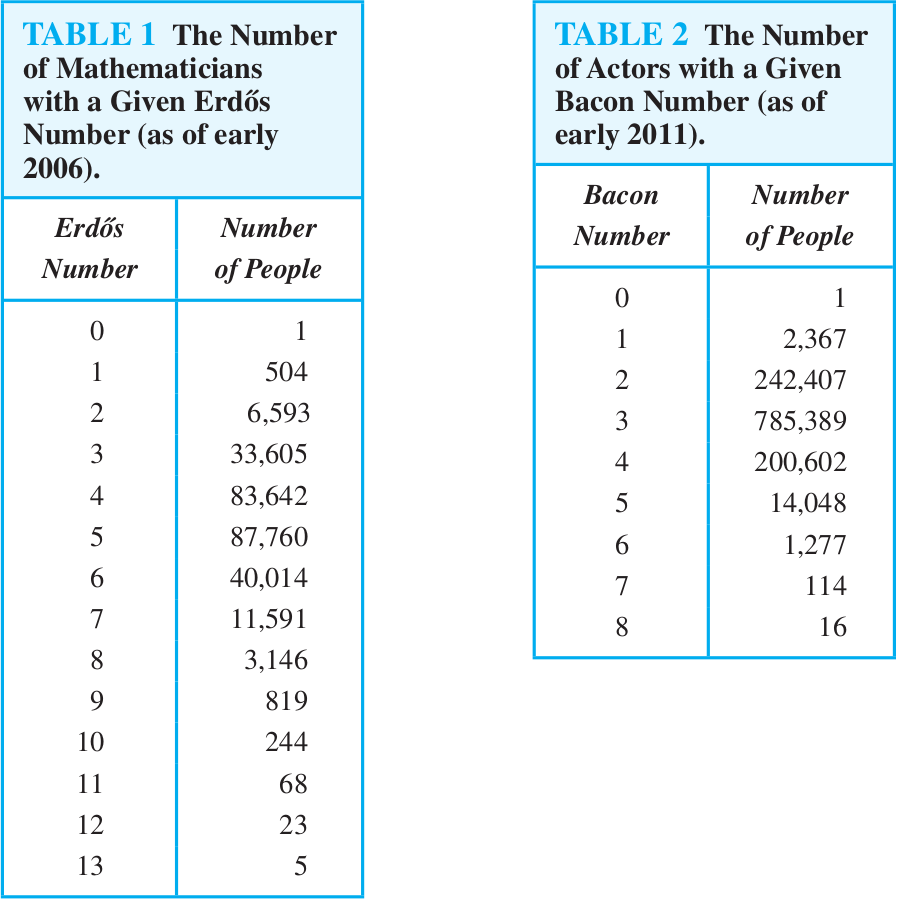
\includegraphics[width=0.7\textwidth]{path-length}
\end{center}
\end{frame}

\section{Samhengi}

\begin{frame}{Samanhangandi net}
Út frá skilgreiningu á vegi fáum við skilgreiningu á samanhangandi (e. \emph{connected}) neti:
\begin{tcolorbox}[title=Samanhangandi net]
Óstefnt net er kallað samanhangandi sé til vegur á milli hverra tveggja aðskildra hnúta í netinu.
\end{tcolorbox}
Af henni má leiða setningu:
\begin{tcolorbox}
Til er einfaldur vegur á milli hverra tveggja aðskildra hnúta í óstefndu samanhangandi neti.
\end{tcolorbox}

\end{frame}

\begin{frame}{Samhengisþættir}
Út frá skilgreiningu á hlutmengi getum við skilgreint hlutnet:
\begin{tcolorbox}[title=Hlutnet]
Hlutnet nets $G$ er net $H$ sem hefur þá eiginleika að hnútamengi $H$ er hlutmengi hnútamengis $G$ og leggjamengi $H$ er hlutmengi leggjamengis $G$.
\end{tcolorbox}
Getum þá skilgreint samhengisþátt:
\begin{tcolorbox}
Samhengisþáttur (e. \emph{connected component}) nets $G$ er hlutnet $G$ sem er samanhangandi og óstækkanlegt.
\end{tcolorbox}
Ósamanhangandi net hefur meira en einn samhengisþátt.
\end{frame}

\begin{frame}{Þrjú net}
\begin{center}
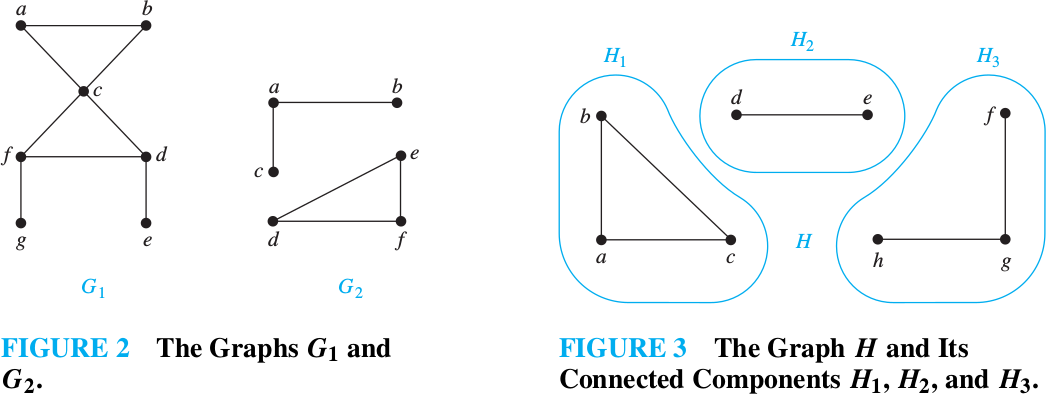
\includegraphics[width=\textwidth]{graph-connectivity}
\end{center}
\end{frame}

\begin{frame}{Brýr}
\begin{tcolorbox}[title=Brú]
Leggur $e$ í $G$ kallast brú (e. \emph{bridge} eða \emph{cut edge}) ef hlutnetið sem myndað er með því að fjarlægja $e$ úr $G$ hefur fleiri samhengisþætti en $G$.
\end{tcolorbox}
Svipaða skilgreiningu má setja fram fyrir hnúta. Slíkir hnútar eru kallaðir ``cut vertices'' í bókinni.
\end{frame}

\begin{frame}{Samhengi}
Við getum skilgreint hnútasamhengi (e. \emph{vertex connectivity}) nets.

\begin{tcolorbox}[title=Samhengi]
Talan $\kappa(G)$ táknar hnútasamhengi netsins $G$. $\kappa(G)$ er lágmarksfjöldi hnúta sem þarf að fjarlægja úr $G$ til að mynda net sem er ósamanhangandi eða með einungis einn hnút.
\end{tcolorbox}
Ósamanhangandi net er með $\kappa(G) = 0$. $\kappa(K_n) = n-1$.
\end{frame}

\begin{frame}{Samhengi og örvanet}
\begin{tcolorbox}[title=Stranglega samanhangandi örvanet]
Örvanet er stranglega samanhangandi (e. \emph{strongly connected}) ef til er örvavegur frá $a$ til $b$ og frá $b$ til $a$ fyrir sérhverja hnúta $a$ og $b$ í örvanetinu.
\end{tcolorbox}

\begin{tcolorbox}[title=Veikt samanhangandi örvanet]
Örvanet er veikt samanhangandi (e. \emph{weakly connected}) sé tilsvarandi óstefnt net samanhangandi.
\end{tcolorbox}
\end{frame}

\begin{frame}{Samanhangandi örvanet}
\begin{center}
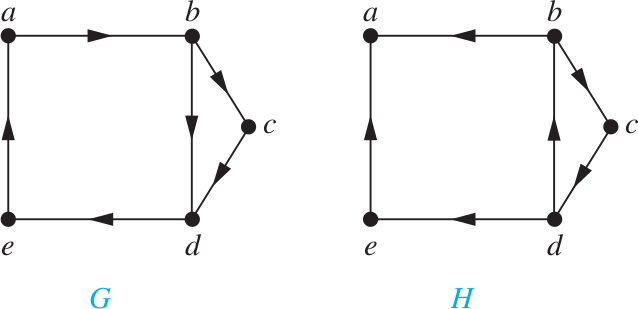
\includegraphics[width=\textwidth]{graph-strong-weak-connected}
\end{center}
\end{frame}
\section{Fjöldi vega}
\begin{frame}{Fjöldi vega}
\begin{tcolorbox}
Látum $G$ vera net með grennslafylkið $A$ m.t.t. hnútaröðunar $v_1, \ldots, v_n$. Þá er fjöldi mismunandi vega af jákvæðri lengd $r$ á milli hnúta $v_i$ og $v_j$ talan sem er í sæti $i,j$ í fylkinu $A^r$.
\end{tcolorbox}
\end{frame}

\begin{frame}{Dæmi}
Finnum fjölda mismunandi vega á milli $a$ og $d$ í eftirfarandi neti:
\begin{columns}
\column{0.25\textwidth}
\begin{center}
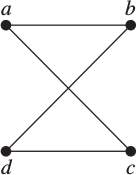
\includegraphics[width=\linewidth]{graph-mini}
\end{center}
\column{0.75\textwidth}
\[
A =
\begin{bmatrix}
0&1&1&0\\
1&0&0&1\\
1&0&0&1\\
0&1&1&0\\
\end{bmatrix}
,
A^4 =
\begin{bmatrix}
8&0&0&8\\
0&8&8&0\\
0&8&8&0\\
8&0&0&8\\
\end{bmatrix}
\]
\begin{center}
Svo fjöldi veganna er 8.
\end{center}
\end{columns}
\end{frame}

\begin{frame}{Næst}
Næst: Förum yfir Euler- og Hamilton-vegi, leit að stystu vegum (kaflar 10.5 og 10.6).
\end{frame}


\end{document}
